\documentclass[10pt, a4paper, notitlepage]{article}
\usepackage{tikz}
\usetikzlibrary{calc}
\usetikzlibrary{cd}
\usetikzlibrary{decorations.markings}
\usetikzlibrary{decorations.pathreplacing}
\usetikzlibrary{decorations.pathmorphing}
\usetikzlibrary{decorations.text}
\usetikzlibrary{arrows.meta}
\usetikzlibrary{arrows}
\usetikzlibrary{positioning}
\usepackage{amssymb}
\usepackage{amsmath}

\begin{document}

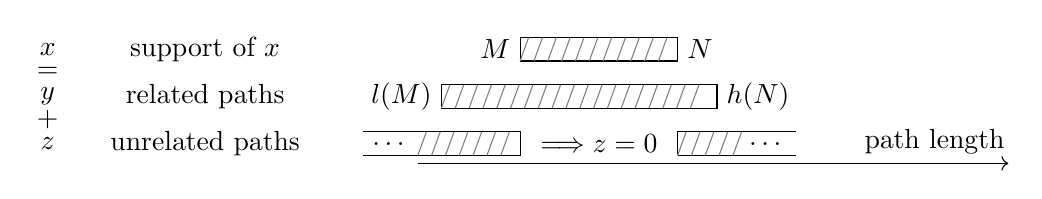
\begin{tikzpicture}
\path[draw] (0, 0) -- ++(up:0.3) node[midway, left] {$ M $} -- ++(right:2) -- ++(down:0.3) node[midway, right] {$ N $} coordinate (top-right) -- ++(left:2) coordinate (top-left);
\path[draw] (-1, -0.6) -- ++(up:0.3) node[midway, left] {$ l(M) $} -- ++(right:3.5) -- ++(down:0.3) node[midway, right] {$ h(N) $} coordinate (mid-right) -- ++(left:3.5) coordinate (mid-left);
\path[draw] (-2, -1.2) ++(up:0.3) coordinate (bot1-dots-top) -- ++(right:2) -- ++(down:0.3) coordinate[midway] (bot1-mid) coordinate (bot1-right) -- ++(left:2) coordinate[pos=0.65] (bot1-left);
\path[draw] (2, -1.2) -- ++(up:0.3) coordinate[midway] (bot2-mid) -- ++(right:1.5) coordinate (bot2-dots-top) ++(down:0.3) coordinate (bot2-dots-bot) [draw] -- ++(left:1.5) coordinate[pos=0.3] (bot2-right) coordinate (bot2-left);
\path ($ (-2, -1.2)!0.5!(bot1-dots-top) $) node[right] {…};
\path ($ (bot2-dots-top)!0.5!(bot2-dots-bot) $) node[left] {…};
\foreach \piece in {top, mid, bot1, bot2} \path[draw, decoration={border, amplitude=9pt, segment length=5pt, angle=70}, decorate, gray] (\piece-left) to (\piece-right);
%
\path[draw, ->] (-1.3, -1.3) to node[very near end, above] {path length} ++(right:7.5);
\path (-4, 0.15) node {support of $ x $};
\path (-4, -0.45) node {related paths};
\path (-4, -1.05) node {unrelated paths};
%
\path (-6, 0.15) node {$ x $};
\path (-6, -0.15) node {$ = $};
\path (-6, -0.45) node {$ y $};
\path (-6, -0.75) node {$ + $};
\path (-6, -1.05) node {$ z $};
\path ($ (bot1-mid)!0.5!(bot2-mid) $) node {$ \Longrightarrow z = 0 $};
\end{tikzpicture}

\end{document}